\documentclass[a4paper, 12pt]{report}
\usepackage{cmap}
\usepackage{amssymb}
\usepackage{amsmath}
\usepackage{graphicx}
\usepackage{amsthm}
\usepackage{upgreek}
\usepackage{setspace}
\usepackage{color}
\usepackage{moreverb}
\usepackage[T2A]{fontenc}
\usepackage[utf8]{inputenc}
\usepackage[normalem]{ulem}
\usepackage{mathtext} % русские буквы в формулах
\usepackage[left=2cm,right=2cm, top=2cm,bottom=2cm,bindingoffset=0cm]{geometry}
\usepackage[english,russian]{babel}
\usepackage[unicode]{hyperref}
\newenvironment{Proof} % имя окружения
{\par\noindent{$\blacklozenge$}} % команды для \begin
{\hfill$\scriptstyle\boxtimes$}
\newcommand{\Rm}{\mathbb{R}}
\newcommand{\Cm}{\mathbb{C}}
\newcommand{\Z}{\mathbb{Z}}
\newcommand{\I}{\mathbb{I}}
\newcommand{\N}{\mathbb{N}}
\newcommand{\rank}{\operatorname{rank}}
\newcommand{\Ra}{\Rightarrow}
\newcommand{\ra}{\rightarrow}
\newcommand{\FI}{\Phi}
\newcommand{\Sp}{\text{Sp}}
\renewcommand{\leq}{\leqslant}
\renewcommand{\geq}{\geqslant}
\renewcommand{\alpha}{\upalpha}
\renewcommand{\beta}{\upbeta}
\renewcommand{\gamma}{\upgamma}
\renewcommand{\delta}{\updelta}
\renewcommand{\varphi}{\upvarphi}
\renewcommand{\phi}{\upvarphi}
\renewcommand{\tau}{\uptau}
\renewcommand{\lambda}{\uplambda}
\renewcommand{\psi}{\uppsi}
\renewcommand{\mu}{\upmu}
\renewcommand{\omega}{\upomega}
\renewcommand{\d}{\partial}
\renewcommand{\xi}{\upxi}
\renewcommand{\epsilon}{\upvarepsilon}
\newcommand{\intx}{\int\limits_{x_0}^x}
\newcommand\Norm[1]{\left\| #1 \right\|}
\newcommand{\sumk}{\sum\limits_{k=0}^\infty}
\newcommand{\sumi}{\sum\limits_{i=0}^\infty}
\newtheorem*{theorem}{Теорема}
\newtheorem*{cor}{Следствие}
\newtheorem*{lem}{Лемма}
\begin{document}
	% Оформление титульного листа
	\begin{titlepage}
		\begin{center}
			\textsc{МИНИСТЕРСТВО ОБРАЗОВАНИЯ РЕСПУБЛИКИ БЕЛАРУСЬ БЕЛОРУССКИЙ ГОСУДАРСТВЕННЫЙ УНИВЕРСИТЕТ
				\\[5mm]
				ФАКУЛЬТЕТ ПРИКЛАДНОЙ МАТЕМАТИКИ И ИНФОРМАТИКИ\\[2mm]
				Кафедра компьютерных технологий и систем
			}
			
			\vfill
			
			\textbf{Отчет по лабораторной работе №2\\
				«Решение смешанных задач для уравнения теплопроводности»\\
				Вариант 9
				\\[26mm]
			}
		\end{center}
		
		\hfill
		\begin{minipage}{.5\textwidth}
			\begin{flushright}
				Пяловой Елизаветы Сергеевны\\
				студентки 3 курса\\
				специальности «прикладная математика»\\[5mm]
				
				Преподаватель:\\[2mm] 
				И. С. Козловская\\
			\end{flushright}
		\end{minipage}%
		\vfill
		\begin{center}
			Минск, 2024\ г.
		\end{center}
	\end{titlepage}
	\newpage
	\section*{Постановка задачи}
	Решить следующую смешанную задачу 
	\begin{equation}
		\begin{cases}
		u_t - u_{xx} = 0,\\
		u|_{x=0} = 1,\\
		u|_{x=l} = 0,\\
		u|_{t=0} = \sin\dfrac{5\pi}{l}x.
	\end{cases}
	\end{equation}
	\section*{Решение задачи в пакете Wolfram Mathematica}
	Перепишем данную задачу в Wolfram Mathematica
	$$
		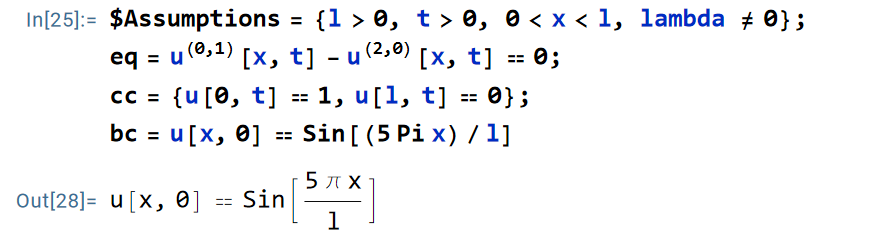
\includegraphics[scale=0.5]{images/img1}
	$$
	Так как уравнение в задаче (1) является однородным, а граничные условия неоднородными, то решение будем искать в виде
	\begin{equation}
		u(x,t) = w(x,t) + v(x,t),
	\end{equation}
	где функцию $w(x,t)$ ищем в виде 
	\begin{equation}
		w(x,t) = a(t)x + b(t).
	\end{equation}
	Необходимо, чтобы функция $w(x,t)$ удовлетворяла граничным условиям
	$$w(0, t) = 1,\ w(l ,t) = 0.$$
	Найдем такую функцию с помощью Wolfram Mathematica
	$$
		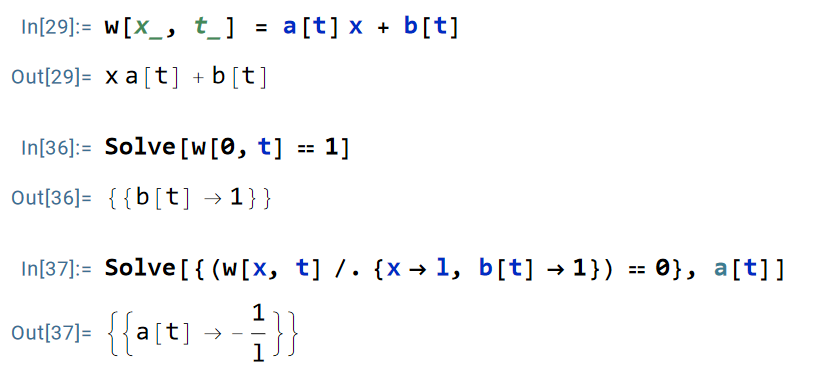
\includegraphics[scale=0.5]{images/img2}
	$$
	то есть \begin{equation}
		w(x,t) = w(x) = 1 - \dfrac xl.
	\end{equation}
	Очевидно, что $w_t = w_{xx} = 0$. В итоге при подстановке решения 
	\begin{equation}
		u(x,t) = 1 - \dfrac xl + v(x,t)
	\end{equation}
	в уравнение задачи (1) мы получим новую задачу с однородными граничными условиями
	\begin{equation}
		\begin{cases}
			v_t - v_{xx} = 0,\\
			v|_{x=0} = 0,\\
			v|_{x=l} = 0,\\
			v|_{t=0} = \sin\dfrac{5\pi}{l}x - 1 + \dfrac x l.
		\end{cases}
	\end{equation}
	В задаче (6) однородное уравнение и однородные граничные условия, поэтому будем искать его решение в виде
	\begin{eqnarray}
		v(x,t) = T(t)X(x),\ T(t)\not\equiv 0, X(x)\not\equiv 0.
	\end{eqnarray}
	Подставим данный вид решения в уравнение задачи (6)
	$$T'(t) X(x) -T(t)X''(x) = 0.$$
	По методу разделения переменных разделим это уравнение на $a^2T(t)X(x)$ и получим
	$$\dfrac{T'(t)}{ T(t)} = \dfrac{X''(x)}{X(x)} = -\lambda^2.$$
	Отсюда получаем два ОДУ
	\begin{eqnarray}
		X''(x) + \lambda^2 X(x) =0,\\
		T'(t) + \lambda^2 T(t) = 0.
	\end{eqnarray}
	Используя граничные условия задачи (6), составим задачу Штурма-Лиувилля для уравнения (8)
	\begin{eqnarray}
	\begin{cases}
	X''(x) + \lambda X(x) = 0,\\
	X(0) = 0,\\
	X(l) = 0.
	\end{cases}
	\end{eqnarray}
	Найдем решение этой задачи в Wolfram Mathematica
	$$
		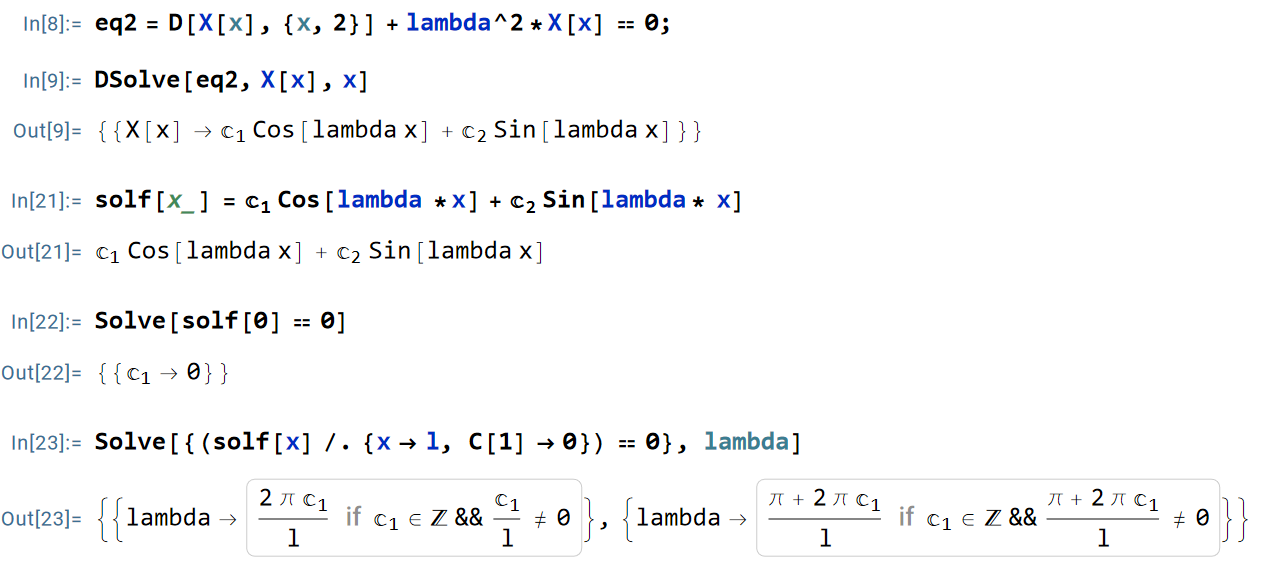
\includegraphics[scale=0.45]{images/img3}
	$$
	то есть 
	\begin{equation}
		\lambda_n = \dfrac{\pi n}{l},\quad X_n(x) = \sin \dfrac{\pi n}{l} x, \quad n = 1,2\ldots.
	\end{equation}
	Найдем общее решение уравнения (9) с помощью Wolfram Mathematica
	$$
		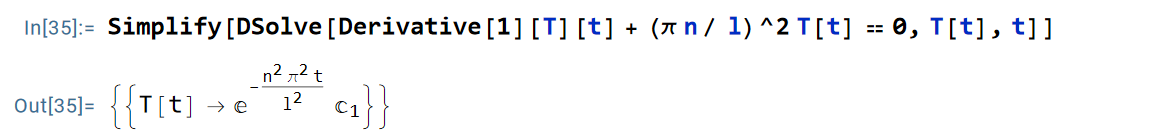
\includegraphics[scale=0.5]{images/img4}
	$$
	то есть \begin{equation}
		T_n(t) = C_1 e^{-\frac{\pi^2 n^2}{l^2}t}.
	\end{equation}
	Подставляем (11) и (12) в общий вид (7) и получим
	\begin{equation}
		v(x,t) = \sum_{n=1}^\infty C_1 e^{-\frac{\pi^2 n^2}{l^2}t}\sin \dfrac{\pi n}{l}x.
	\end{equation}
	Подставляя в (13) начальное условие задачи (6), получим
	$$\sum_{n=1}^\infty C_1 \sin \dfrac{\pi n}{l}x = \sin\dfrac{5\pi}{l}x-1 + \dfrac{x}{l},$$
	то есть $C_1$ --- это коэффициент разложения функции справа в ряд Фурье по собственным функциям
	$$C_1 = \dfrac{2}{l}\int\limits_0^l\left(\sin\dfrac{5\pi}{l}x-1 + \dfrac{x}{l} \right)\sin\dfrac{\pi n}{l}xdx.$$
	Найдем значение этого интеграла с помощью Wolfram Mathematica
	$$
		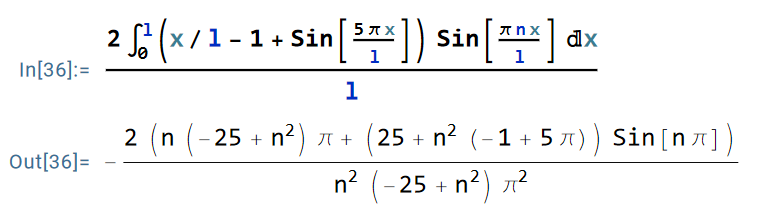
\includegraphics[scale=0.5]{images/img5}
	$$
	Поскольку $\sin \pi n = 0$, то, сократив, получим
	\begin{equation}
		C_1 = -\dfrac{2}{\pi n}.
	\end{equation}
	Подставим (14) в (13) и получим 
	\begin{equation}
		v(x,t) = \sum_{n=1}^\infty -\dfrac{2}{\pi n} e^{-\frac{\pi^2 n^2}{l^2}t}\sin \dfrac{\pi n}{l}x.
	\end{equation}
	Складывая (4) и (15) в соответствии с (2), получим итоговый вид решения задачи (1)
	\begin{equation}
		u(x,t) = 1 - \dfrac x l + \sum_{n=1}^\infty -\dfrac{2}{\pi n} e^{-\frac{\pi^2 n^2}{l^2}t}\sin \dfrac{\pi n}{l}x.
	\end{equation}
	Для проверки подставим $n$-ое слагаемое суммы (16) в задачу (1)
	$$
		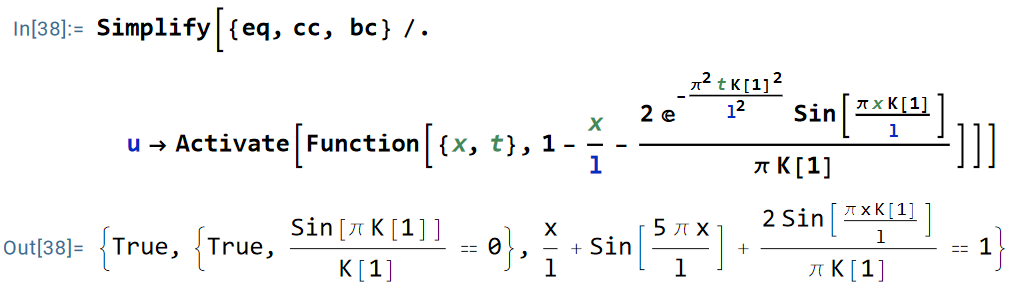
\includegraphics[scale=0.5]{images/img6}
	$$
	то есть $T_n(t)X_n(x)$ удовлетворяют уравнению и граничным условиям (второе условие также выполнено, так как $\sin \pi n = 0$). Для третьего условия получилось равенство $$\dfrac xl -1 +\sin\dfrac{5\pi}{l}x = - \dfrac2 {\pi n} \sin \dfrac{\pi n}{l},$$
	где значение справа соответствует одному из коэффициентов разложения в ряд Фурье функции слева, то есть условие тоже выполняется (если бы мы подставляли бесконечную сумму).
	Таким образом, решение задачи (1) задано функцией.\\\\
	Теперь найдем решение задачи (1) через команду DSolve
	$$
		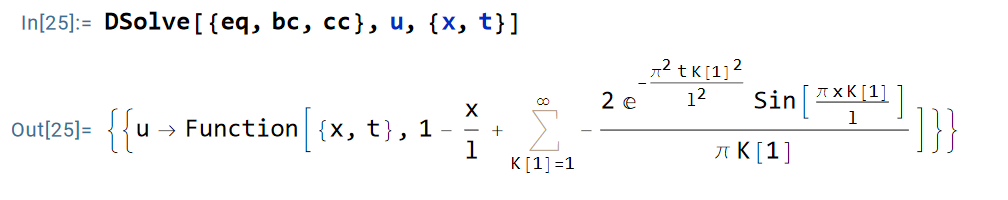
\includegraphics[scale=0.4]{images/img7}
	$$
	что совпадает с построенным нами решением.
\section*{Вывод}
Таким образом, мы нашли решение смешанной задачи для уравнения теплопроводности методом разделения переменных, а затем проверили, правильно ли оно было вычислено, с помощью Wolfram Mathematica.
\end{document}

 